

\section{Results and Discussion}
The analysis and calculations were conducted using the R programming language \cite{R} and Python Jupyter Notebooks \cite{IPython:2007}. The scripts are included in the appendix of this report. \ref{r_scripts} All uncertainties stated are provided for a 95 \% confidence interval. The uncertainties were modelled with the aid of \texttt{METAS UncLib}, a Python uncertainty modelling library by the Swiss institute of metrology METAS.\cite{unclib}


\subsection{Calibration}

Measuring the temperature response from the system while heating well-defined \qty{100}{\milli\liter} of water and using (\ref{eq:4}) yields a net heat capacity of the empty dewar of \qty{163 \pm 8}{\joule\per\kelvin}.


\subsection{Specific heat capacity of ethanol/water mixture}

Running the same procedure for a liquid with unknown heat capacity allows deriving the heat capacity of the solution itself by deducting the dewars heat capacity from the heat capacity of the entire system. The latter was determined thorugh calibration.The entire laboratory collaborated to measure the specific heat capacity of ethanol water mixtures. The authors' mixtures contained \qty{80.09}{\percent}, \qty{88.86}{\percent} and \qty{93.73}{\percent} of ethanol respectively (mass percent). Specific heat capacities of \qty{2920 \pm 100}{\joule\per\kelvin\per\kilo\gram}, \qty{2590 \pm 100}{\joule\per\kelvin\per\kilo\gram} and \qty{2430 \pm 100}{\joule\per\kelvin\per\kilo\gram} were found. This corresponds well with literature values of \qty{2900}{\joule\per\kelvin\per\kilo\gram}, \qty{2700}{\joule\per\kelvin\per\kilo\gram} and \qty{2560}{\joule\per\kelvin\per\kilo\gram}.

The uncertainties for these measurements were derived from the standard deviation of the system calibration, since the scattering in the raw data can be assumed the same for ethanol and for water.


\begin{figure}[H]
    \centering
    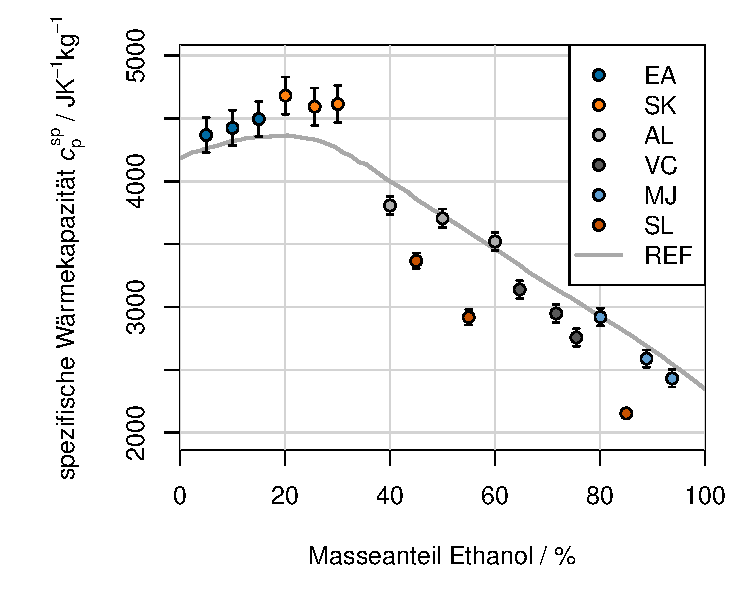
\includegraphics[width=.5\textwidth]{figures/plots/ethanol_alldata_5_4_in.pdf}
    \caption{The specific heat capacity $c^{sp}_p$ as a function of the ethanol share in water. The grey line represents literature values\cite{ethanol_water}, the coloured dots show the values obtained by the teams, indicated by their initials. Our values are the blue ones on the right-hand side labelled "MJ".}
    \label{fig:eth_all}
\end{figure}


\subsection{Solution enthalpy of ammonium nitrate}

By comparing the temperature drop caused by dissolving \qty{600}{\milli\gram} of \ce{NH_4NO_3} with the rise in temperature upon heating and using (\ref{eq:6}) as well as the knowledge of the systems heat capacity garnered through calibration, the solution enthalpy of ammonium nitrate was calculated at $\Delta_{sol}H_{\mathrm{NH_4NO_3}} = $ \qty{29.0 \pm 1.6}{\kilo\joule\per\mole}. 


\begin{figure}[H]
    \centering
    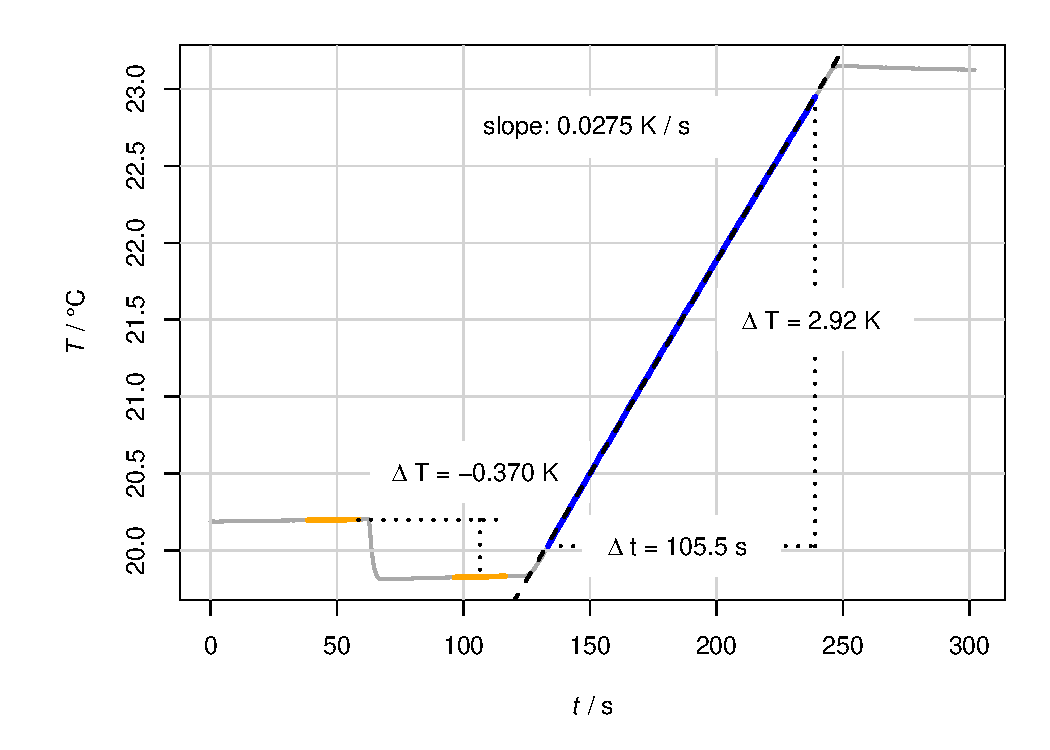
\includegraphics[width=.5\textwidth]{figures/plots/sol3.pdf}
    \caption{An example of the data recorded for the determination of the solution enthalpy of ammonium nitrate. The orange lines were read out for the temperature drop of dissolution, the blue slope was used as calibration reference. This procedure was identically repeated three times.}
    \label{fig:sol3}
\end{figure}



\subsection{Calorimetric titration of vinegar}

\begin{figure}[H]
    \centering
    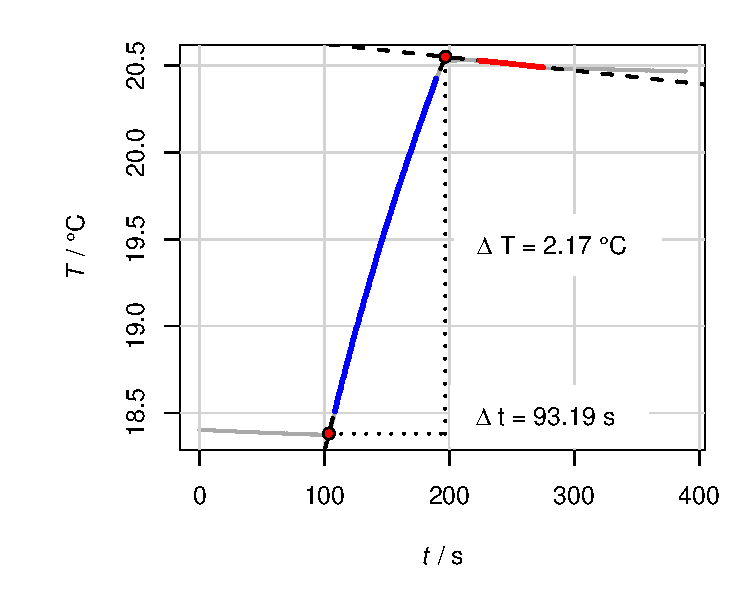
\includegraphics[width=.5\textwidth]{figures/plots/vinegar_cont.pdf}
    \caption{Continuous titration of vinegar with sodium hydroxide.}
    \label{fig:vinegar_cont}
\end{figure}

\begin{figure}[H]
    \centering
    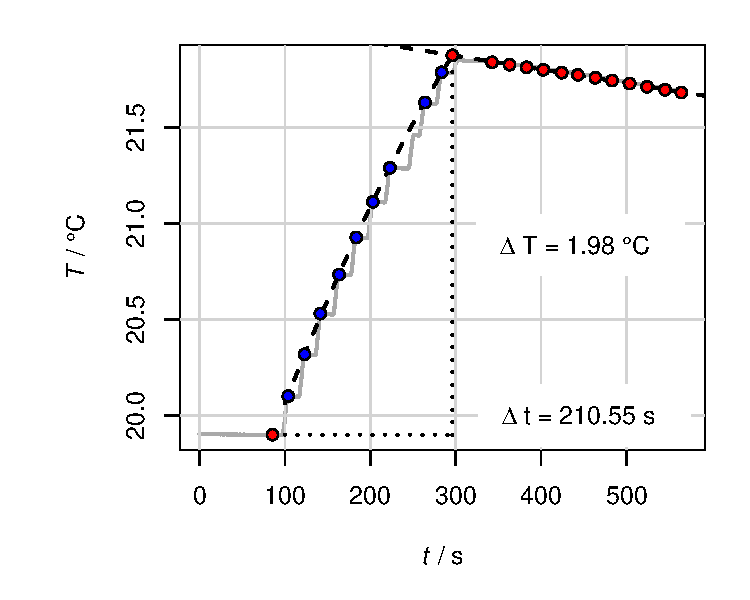
\includegraphics[width=.5\textwidth]{figures/plots/vinegar_uncont.pdf}
    \caption{Discrete titration of vinegar with sodium hydroxide. A high resolution version of this plot can be found in the appendix.\ref{fig:vinegar_uncont_highres}}
    \label{fig:vinegar_uncont}
\end{figure}

By calorimetric titration with \ce{NaOH}, the acetate concentration of a vinegar sample was found to be \qty{0.8283 \pm 0.0018}{\M} with continuous titration and \qty{0.842 \pm 0.018}{\M} with stepwise titration. This converts to \qty{49.74 \pm 0.11}{\gram\per\liter} and \qty{50.6 \pm 1.2}{\gram\per\liter} of acetic acid respectively.



\subsection{Melting enthalpy of ice}

From measuring the temperature drop of well-defined amounts of water and ice three times each, a melting enthalpy of \qty{330 \pm 50}{\kilo\joule\per\kilo\gram} was determined. This corresponds well with the literature value of \qty{333.55}{\kilo\joule\per\kilo\gram}.\cite{crc}


